\documentclass[twoside]{book}

% Packages required by doxygen
\usepackage{calc}
\usepackage{doxygen}
\usepackage{graphicx}
\usepackage[utf8]{inputenc}
\usepackage{makeidx}
\usepackage{multicol}
\usepackage{multirow}
\usepackage{textcomp}
\usepackage[table]{xcolor}

% Font selection
\usepackage[T1]{fontenc}
\usepackage{mathptmx}
\usepackage[scaled=.90]{helvet}
\usepackage{courier}
\usepackage{amssymb}
\usepackage{sectsty}
\renewcommand{\familydefault}{\sfdefault}
\allsectionsfont{%
  \fontseries{bc}\selectfont%
  \color{darkgray}%
}
\renewcommand{\DoxyLabelFont}{%
  \fontseries{bc}\selectfont%
  \color{darkgray}%
}

% Page & text layout
\usepackage{geometry}
\geometry{%
  a4paper,%
  top=2.5cm,%
  bottom=2.5cm,%
  left=2.5cm,%
  right=2.5cm%
}
\tolerance=750
\hfuzz=15pt
\hbadness=750
\setlength{\emergencystretch}{15pt}
\setlength{\parindent}{0cm}
\setlength{\parskip}{0.2cm}
\makeatletter
\renewcommand{\paragraph}{%
  \@startsection{paragraph}{4}{0ex}{-1.0ex}{1.0ex}{%
    \normalfont\normalsize\bfseries\SS@parafont%
  }%
}
\renewcommand{\subparagraph}{%
  \@startsection{subparagraph}{5}{0ex}{-1.0ex}{1.0ex}{%
    \normalfont\normalsize\bfseries\SS@subparafont%
  }%
}
\makeatother

% Headers & footers
\usepackage{fancyhdr}
\pagestyle{fancyplain}
\fancyhead[LE]{\fancyplain{}{\bfseries\thepage}}
\fancyhead[CE]{\fancyplain{}{}}
\fancyhead[RE]{\fancyplain{}{\bfseries\leftmark}}
\fancyhead[LO]{\fancyplain{}{\bfseries\rightmark}}
\fancyhead[CO]{\fancyplain{}{}}
\fancyhead[RO]{\fancyplain{}{\bfseries\thepage}}
\fancyfoot[LE]{\fancyplain{}{}}
\fancyfoot[CE]{\fancyplain{}{}}
\fancyfoot[RE]{\fancyplain{}{\bfseries\scriptsize Generated on Mon Oct 21 2013 13\-:40\-:41 for My Project by Doxygen }}
\fancyfoot[LO]{\fancyplain{}{\bfseries\scriptsize Generated on Mon Oct 21 2013 13\-:40\-:41 for My Project by Doxygen }}
\fancyfoot[CO]{\fancyplain{}{}}
\fancyfoot[RO]{\fancyplain{}{}}
\renewcommand{\footrulewidth}{0.4pt}
\renewcommand{\chaptermark}[1]{%
  \markboth{#1}{}%
}
\renewcommand{\sectionmark}[1]{%
  \markright{\thesection\ #1}%
}

% Indices & bibliography
\usepackage{natbib}
\usepackage[titles]{tocloft}
\setcounter{tocdepth}{3}
\setcounter{secnumdepth}{5}
\makeindex

% Hyperlinks (required, but should be loaded last)
\usepackage{ifpdf}
\ifpdf
  \usepackage[pdftex,pagebackref=true]{hyperref}
\else
  \usepackage[ps2pdf,pagebackref=true]{hyperref}
\fi
\hypersetup{%
  colorlinks=true,%
  linkcolor=blue,%
  citecolor=blue,%
  unicode%
}

% Custom commands
\newcommand{\clearemptydoublepage}{%
  \newpage{\pagestyle{empty}\cleardoublepage}%
}


%===== C O N T E N T S =====

\begin{document}

% Titlepage & ToC
\hypersetup{pageanchor=false}
\pagenumbering{roman}
\begin{titlepage}
\vspace*{7cm}
\begin{center}%
{\Large My Project }\\
\vspace*{1cm}
{\large Generated by Doxygen 1.8.5}\\
\vspace*{0.5cm}
{\small Mon Oct 21 2013 13:40:41}\\
\end{center}
\end{titlepage}
\clearemptydoublepage
\tableofcontents
\clearemptydoublepage
\pagenumbering{arabic}
\hypersetup{pageanchor=true}

%--- Begin generated contents ---
\chapter{Hierarchical Index}
\section{Class Hierarchy}
This inheritance list is sorted roughly, but not completely, alphabetically\-:\begin{DoxyCompactList}
\item C\-C\-Application\begin{DoxyCompactList}
\item \contentsline{section}{App\-Delegate}{\pageref{class_app_delegate}}{}
\end{DoxyCompactList}
\item C\-C\-Layer\begin{DoxyCompactList}
\item \contentsline{section}{J\-G\-\_\-\-Main\-\_\-\-Game}{\pageref{class_j_g___main___game}}{}
\item \contentsline{section}{J\-G\-\_\-\-Main\-\_\-\-Menu}{\pageref{class_j_g___main___menu}}{}
\end{DoxyCompactList}
\item C\-C\-Node\begin{DoxyCompactList}
\item \contentsline{section}{J\-G\-\_\-\-Temp\-Line\-Container}{\pageref{class_j_g___temp_line_container}}{}
\end{DoxyCompactList}
\item C\-C\-Sprite\begin{DoxyCompactList}
\item \contentsline{section}{J\-G\-\_\-\-Ball}{\pageref{class_j_g___ball}}{}
\item \contentsline{section}{J\-G\-\_\-\-Bonus\-\_\-\-Base}{\pageref{class_j_g___bonus___base}}{}
\item \contentsline{section}{J\-G\-\_\-\-Hand}{\pageref{class_j_g___hand}}{}
\end{DoxyCompactList}
\end{DoxyCompactList}

\chapter{Class Index}
\section{Class List}
Here are the classes, structs, unions and interfaces with brief descriptions\-:\begin{DoxyCompactList}
\item\contentsline{section}{\hyperlink{class_app_delegate}{App\-Delegate} }{\pageref{class_app_delegate}}{}
\item\contentsline{section}{\hyperlink{class_j_g___ball}{J\-G\-\_\-\-Ball} }{\pageref{class_j_g___ball}}{}
\item\contentsline{section}{\hyperlink{class_j_g___bonus___base}{J\-G\-\_\-\-Bonus\-\_\-\-Base} }{\pageref{class_j_g___bonus___base}}{}
\item\contentsline{section}{\hyperlink{class_j_g___game___h_u_d}{J\-G\-\_\-\-Game\-\_\-\-H\-U\-D} }{\pageref{class_j_g___game___h_u_d}}{}
\item\contentsline{section}{\hyperlink{class_j_g___game___main}{J\-G\-\_\-\-Game\-\_\-\-Main} }{\pageref{class_j_g___game___main}}{}
\item\contentsline{section}{\hyperlink{class_j_g___hand}{J\-G\-\_\-\-Hand} }{\pageref{class_j_g___hand}}{}
\item\contentsline{section}{\hyperlink{class_j_g___menu___main}{J\-G\-\_\-\-Menu\-\_\-\-Main} }{\pageref{class_j_g___menu___main}}{}
\item\contentsline{section}{\hyperlink{struct_s_touch_info}{S\-Touch\-Info} }{\pageref{struct_s_touch_info}}{}
\item\contentsline{section}{\hyperlink{structtag_resource}{tag\-Resource} \\*The cocos2d Application }{\pageref{structtag_resource}}{}
\end{DoxyCompactList}

\chapter{Class Documentation}
\hypertarget{class_app_delegate}{\section{App\-Delegate Class Reference}
\label{class_app_delegate}\index{App\-Delegate@{App\-Delegate}}
}
Inheritance diagram for App\-Delegate\-:\begin{figure}[H]
\begin{center}
\leavevmode
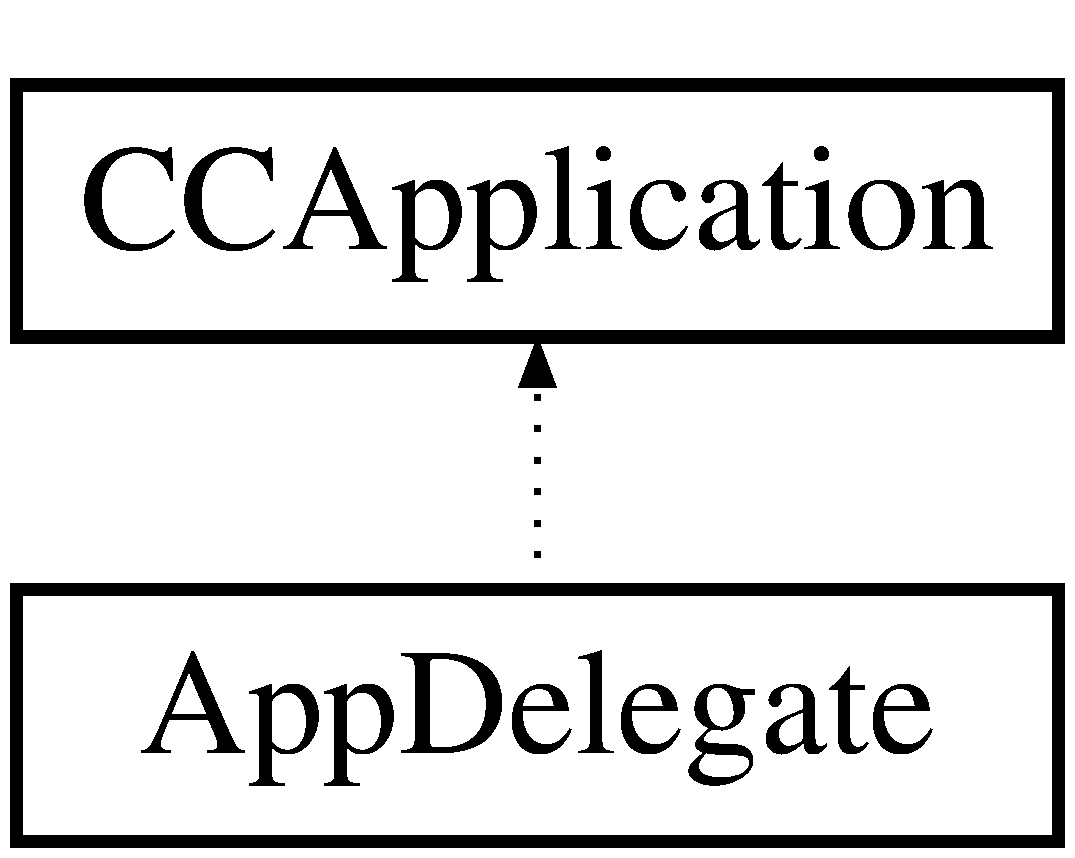
\includegraphics[height=2.000000cm]{class_app_delegate}
\end{center}
\end{figure}
\subsection*{Public Member Functions}
\begin{DoxyCompactItemize}
\item 
virtual bool \hyperlink{class_app_delegate_a68cbaed49edf7581dc59a09d5062fff3}{application\-Did\-Finish\-Launching} ()
\begin{DoxyCompactList}\small\item\em Implement C\-C\-Director and C\-C\-Scene init code here. \end{DoxyCompactList}\item 
virtual void \hyperlink{class_app_delegate_a17cb09777419781698324e0415bffd3a}{application\-Did\-Enter\-Background} ()
\begin{DoxyCompactList}\small\item\em The function be called when the application enter background. \end{DoxyCompactList}\item 
virtual void \hyperlink{class_app_delegate_ac4d653e3f74a91efef5f2def58fe3108}{application\-Will\-Enter\-Foreground} ()
\begin{DoxyCompactList}\small\item\em The function be called when the application enter foreground. \end{DoxyCompactList}\end{DoxyCompactItemize}


\subsection{Member Function Documentation}
\hypertarget{class_app_delegate_a17cb09777419781698324e0415bffd3a}{\index{App\-Delegate@{App\-Delegate}!application\-Did\-Enter\-Background@{application\-Did\-Enter\-Background}}
\index{application\-Did\-Enter\-Background@{application\-Did\-Enter\-Background}!AppDelegate@{App\-Delegate}}
\subsubsection[{application\-Did\-Enter\-Background}]{\setlength{\rightskip}{0pt plus 5cm}void App\-Delegate\-::application\-Did\-Enter\-Background (
\begin{DoxyParamCaption}
{}
\end{DoxyParamCaption}
)\hspace{0.3cm}{\ttfamily [virtual]}}}\label{class_app_delegate_a17cb09777419781698324e0415bffd3a}


The function be called when the application enter background. 


\begin{DoxyParams}{Parameters}
{\em the} & pointer of the application \\
\hline
\end{DoxyParams}
\hypertarget{class_app_delegate_a68cbaed49edf7581dc59a09d5062fff3}{\index{App\-Delegate@{App\-Delegate}!application\-Did\-Finish\-Launching@{application\-Did\-Finish\-Launching}}
\index{application\-Did\-Finish\-Launching@{application\-Did\-Finish\-Launching}!AppDelegate@{App\-Delegate}}
\subsubsection[{application\-Did\-Finish\-Launching}]{\setlength{\rightskip}{0pt plus 5cm}bool App\-Delegate\-::application\-Did\-Finish\-Launching (
\begin{DoxyParamCaption}
{}
\end{DoxyParamCaption}
)\hspace{0.3cm}{\ttfamily [virtual]}}}\label{class_app_delegate_a68cbaed49edf7581dc59a09d5062fff3}


Implement C\-C\-Director and C\-C\-Scene init code here. 

\begin{DoxyReturn}{Returns}
true Initialize success, app continue. 

false Initialize failed, app terminate. 
\end{DoxyReturn}
\hypertarget{class_app_delegate_ac4d653e3f74a91efef5f2def58fe3108}{\index{App\-Delegate@{App\-Delegate}!application\-Will\-Enter\-Foreground@{application\-Will\-Enter\-Foreground}}
\index{application\-Will\-Enter\-Foreground@{application\-Will\-Enter\-Foreground}!AppDelegate@{App\-Delegate}}
\subsubsection[{application\-Will\-Enter\-Foreground}]{\setlength{\rightskip}{0pt plus 5cm}void App\-Delegate\-::application\-Will\-Enter\-Foreground (
\begin{DoxyParamCaption}
{}
\end{DoxyParamCaption}
)\hspace{0.3cm}{\ttfamily [virtual]}}}\label{class_app_delegate_ac4d653e3f74a91efef5f2def58fe3108}


The function be called when the application enter foreground. 


\begin{DoxyParams}{Parameters}
{\em the} & pointer of the application \\
\hline
\end{DoxyParams}


The documentation for this class was generated from the following files\-:\begin{DoxyCompactItemize}
\item 
App\-Delegate.\-h\item 
App\-Delegate.\-cpp\end{DoxyCompactItemize}

\hypertarget{class_j_g___ball}{\section{J\-G\-\_\-\-Ball Class Reference}
\label{class_j_g___ball}\index{J\-G\-\_\-\-Ball@{J\-G\-\_\-\-Ball}}
}


{\ttfamily \#include $<$J\-G\-\_\-\-Ball.\-h$>$}

Inheritance diagram for J\-G\-\_\-\-Ball\-:\begin{figure}[H]
\begin{center}
\leavevmode
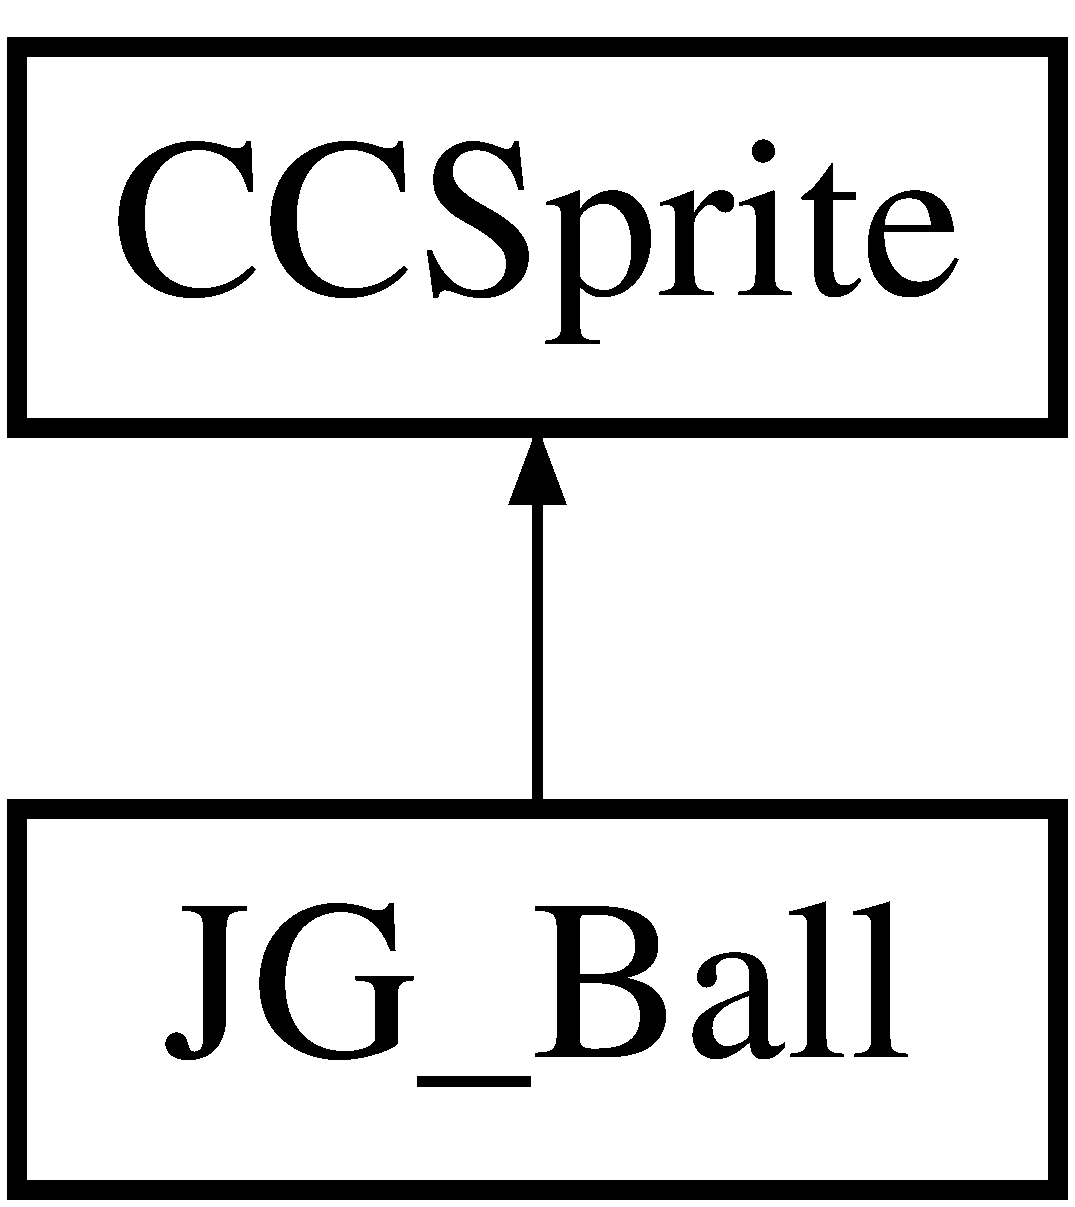
\includegraphics[height=2.000000cm]{class_j_g___ball}
\end{center}
\end{figure}
\subsection*{Public Member Functions}
\begin{DoxyCompactItemize}
\item 
void \hyperlink{class_j_g___ball_a601eda0b1aaf9d4c8fdd31d36234a6c1}{Move\-Curve} (float force, C\-C\-Point destination)
\item 
void \hyperlink{class_j_g___ball_afa347dae4a20695cf506375b798cb2f3}{Move\-Staight} (float force, C\-C\-Point destination)
\item 
void \hyperlink{class_j_g___ball_a21c06d1a10aa8fdcc3d8e63a82f221fe}{update} (float dt)
\item 
\hypertarget{class_j_g___ball_adb4350ed0da24e5499c3402bc322f559}{void {\bfseries temp\-Reset} ()}\label{class_j_g___ball_adb4350ed0da24e5499c3402bc322f559}

\item 
E\-Throw\-Direction \hyperlink{class_j_g___ball_a94843b91ab6f8cddbb2b90de6daeb531}{Get\-Ball\-Direction} ()
\item 
\hypertarget{class_j_g___ball_a0ad42506b43718f14ccb45f163d92999}{C\-C\-Point {\bfseries Get\-Initial\-Touch\-Position} ()}\label{class_j_g___ball_a0ad42506b43718f14ccb45f163d92999}

\item 
\hypertarget{class_j_g___ball_a628e6f457315f1af9d9638834dff91e0}{void {\bfseries Set\-Initial\-Touch\-Position} (C\-C\-Point new\-Touch\-Pos)}\label{class_j_g___ball_a628e6f457315f1af9d9638834dff91e0}

\end{DoxyCompactItemize}
\subsection*{Static Public Member Functions}
\begin{DoxyCompactItemize}
\item 
static \hyperlink{class_j_g___ball}{J\-G\-\_\-\-Ball} $\ast$ \hyperlink{class_j_g___ball_a12279a500446c9516026d3f52fee87eb}{create\-With\-File\-Name} (const char $\ast$psz\-File\-Name, C\-C\-Point initial\-Pos)
\item 
static void \hyperlink{class_j_g___ball_a8023f3c38c257dd4430a5a01c519a289}{Calculate\-Speed\-Boundries\-Base\-On\-Length} (float delta\-X)
\end{DoxyCompactItemize}
\subsection*{Public Attributes}
\begin{DoxyCompactItemize}
\item 
\hypertarget{class_j_g___ball_ad4aa2855022e5315addf40ef73ee6972}{float {\bfseries speed}}\label{class_j_g___ball_ad4aa2855022e5315addf40ef73ee6972}

\item 
\hypertarget{class_j_g___ball_a743ed73473f38e9466f305c3f8efe995}{E\-Throw\-Direction {\bfseries ball\-Throw\-Direction}}\label{class_j_g___ball_a743ed73473f38e9466f305c3f8efe995}

\item 
\hypertarget{class_j_g___ball_af0bd7eeacc5d8f094d921663843b5179}{float {\bfseries curve\-\_\-\-Total\-Time}}\label{class_j_g___ball_af0bd7eeacc5d8f094d921663843b5179}

\item 
\hypertarget{class_j_g___ball_a681ecc9587d2d8d857f656d19d297ef8}{float {\bfseries curve\-\_\-\-Y0}}\label{class_j_g___ball_a681ecc9587d2d8d857f656d19d297ef8}

\item 
\hypertarget{class_j_g___ball_a8dcbff9b6d7f9f8737b3421f26c699e7}{float {\bfseries curve\-\_\-\-X0}}\label{class_j_g___ball_a8dcbff9b6d7f9f8737b3421f26c699e7}

\item 
\hypertarget{class_j_g___ball_a32222cd24992fff289361884db472b23}{float {\bfseries curve\-\_\-\-Rad}}\label{class_j_g___ball_a32222cd24992fff289361884db472b23}

\item 
\hypertarget{class_j_g___ball_a399ae1fb026df3759d3616c7b74eecaa}{float {\bfseries straight\-\_\-\-Dir}}\label{class_j_g___ball_a399ae1fb026df3759d3616c7b74eecaa}

\item 
\hypertarget{class_j_g___ball_a2cab0645b2eb4374fbfde0b0399c0e72}{C\-C\-Point {\bfseries temp\-Initial\-Position}}\label{class_j_g___ball_a2cab0645b2eb4374fbfde0b0399c0e72}

\item 
\hypertarget{class_j_g___ball_a358259dea815fa262327e0af48a6af3c}{E\-Throw\-Direction {\bfseries temp\-Initial\-Throw\-Direction}}\label{class_j_g___ball_a358259dea815fa262327e0af48a6af3c}

\item 
\hypertarget{class_j_g___ball_a602558390080ce6d8cdfcfdbc09f7b12}{C\-C\-Repeat\-Forever $\ast$ {\bfseries action\-\_\-\-Rotate}}\label{class_j_g___ball_a602558390080ce6d8cdfcfdbc09f7b12}

\item 
\hypertarget{class_j_g___ball_aa0fc27312d724fcf2324e87844a99cb8}{\hyperlink{class_j_g___temp_line_container}{J\-G\-\_\-\-Temp\-Line\-Container} $\ast$ {\bfseries temp\-Draw}}\label{class_j_g___ball_aa0fc27312d724fcf2324e87844a99cb8}

\item 
\hypertarget{class_j_g___ball_aacc0e044d12a3fe88d03b54f8c800626}{C\-C\-Point {\bfseries touch\-Position}}\label{class_j_g___ball_aacc0e044d12a3fe88d03b54f8c800626}

\item 
\hypertarget{class_j_g___ball_a0ad0f2f4b8d03d63c879544111a24506}{E\-Move\-Mode {\bfseries move\-Mode}}\label{class_j_g___ball_a0ad0f2f4b8d03d63c879544111a24506}

\end{DoxyCompactItemize}
\subsection*{Static Public Attributes}
\begin{DoxyCompactItemize}
\item 
\hypertarget{class_j_g___ball_a0e5845ccdb93030b567b796f6266e517}{static float {\bfseries min\-Speed}}\label{class_j_g___ball_a0e5845ccdb93030b567b796f6266e517}

\item 
\hypertarget{class_j_g___ball_ad830251662cdf8443962aef638ffefcc}{static float {\bfseries max\-Speed}}\label{class_j_g___ball_ad830251662cdf8443962aef638ffefcc}

\end{DoxyCompactItemize}


\subsection{Detailed Description}
class for handling ball 

\subsection{Member Function Documentation}
\hypertarget{class_j_g___ball_a8023f3c38c257dd4430a5a01c519a289}{\index{J\-G\-\_\-\-Ball@{J\-G\-\_\-\-Ball}!Calculate\-Speed\-Boundries\-Base\-On\-Length@{Calculate\-Speed\-Boundries\-Base\-On\-Length}}
\index{Calculate\-Speed\-Boundries\-Base\-On\-Length@{Calculate\-Speed\-Boundries\-Base\-On\-Length}!JG_Ball@{J\-G\-\_\-\-Ball}}
\subsubsection[{Calculate\-Speed\-Boundries\-Base\-On\-Length}]{\setlength{\rightskip}{0pt plus 5cm}static void J\-G\-\_\-\-Ball\-::\-Calculate\-Speed\-Boundries\-Base\-On\-Length (
\begin{DoxyParamCaption}
\item[{float}]{delta\-X}
\end{DoxyParamCaption}
)\hspace{0.3cm}{\ttfamily [inline]}, {\ttfamily [static]}}}\label{class_j_g___ball_a8023f3c38c257dd4430a5a01c519a289}
Calculate the minimum Speed , based on the distance of handes \hypertarget{class_j_g___ball_a12279a500446c9516026d3f52fee87eb}{\index{J\-G\-\_\-\-Ball@{J\-G\-\_\-\-Ball}!create\-With\-File\-Name@{create\-With\-File\-Name}}
\index{create\-With\-File\-Name@{create\-With\-File\-Name}!JG_Ball@{J\-G\-\_\-\-Ball}}
\subsubsection[{create\-With\-File\-Name}]{\setlength{\rightskip}{0pt plus 5cm}{\bf J\-G\-\_\-\-Ball} $\ast$ J\-G\-\_\-\-Ball\-::create\-With\-File\-Name (
\begin{DoxyParamCaption}
\item[{const char $\ast$}]{psz\-File\-Name, }
\item[{C\-C\-Point}]{initial\-Pos}
\end{DoxyParamCaption}
)\hspace{0.3cm}{\ttfamily [static]}}}\label{class_j_g___ball_a12279a500446c9516026d3f52fee87eb}
Creating ball in a specific position \hypertarget{class_j_g___ball_a94843b91ab6f8cddbb2b90de6daeb531}{\index{J\-G\-\_\-\-Ball@{J\-G\-\_\-\-Ball}!Get\-Ball\-Direction@{Get\-Ball\-Direction}}
\index{Get\-Ball\-Direction@{Get\-Ball\-Direction}!JG_Ball@{J\-G\-\_\-\-Ball}}
\subsubsection[{Get\-Ball\-Direction}]{\setlength{\rightskip}{0pt plus 5cm}E\-Throw\-Direction J\-G\-\_\-\-Ball\-::\-Get\-Ball\-Direction (
\begin{DoxyParamCaption}
{}
\end{DoxyParamCaption}
)\hspace{0.3cm}{\ttfamily [inline]}}}\label{class_j_g___ball_a94843b91ab6f8cddbb2b90de6daeb531}
get the direction of ball \hypertarget{class_j_g___ball_a601eda0b1aaf9d4c8fdd31d36234a6c1}{\index{J\-G\-\_\-\-Ball@{J\-G\-\_\-\-Ball}!Move\-Curve@{Move\-Curve}}
\index{Move\-Curve@{Move\-Curve}!JG_Ball@{J\-G\-\_\-\-Ball}}
\subsubsection[{Move\-Curve}]{\setlength{\rightskip}{0pt plus 5cm}void J\-G\-\_\-\-Ball\-::\-Move\-Curve (
\begin{DoxyParamCaption}
\item[{float}]{force, }
\item[{C\-C\-Point}]{destination}
\end{DoxyParamCaption}
)}}\label{class_j_g___ball_a601eda0b1aaf9d4c8fdd31d36234a6c1}
Initial the curve movement variables \hypertarget{class_j_g___ball_afa347dae4a20695cf506375b798cb2f3}{\index{J\-G\-\_\-\-Ball@{J\-G\-\_\-\-Ball}!Move\-Staight@{Move\-Staight}}
\index{Move\-Staight@{Move\-Staight}!JG_Ball@{J\-G\-\_\-\-Ball}}
\subsubsection[{Move\-Staight}]{\setlength{\rightskip}{0pt plus 5cm}void J\-G\-\_\-\-Ball\-::\-Move\-Staight (
\begin{DoxyParamCaption}
\item[{float}]{force, }
\item[{C\-C\-Point}]{destination}
\end{DoxyParamCaption}
)}}\label{class_j_g___ball_afa347dae4a20695cf506375b798cb2f3}
Initial the straight movement variables \hypertarget{class_j_g___ball_a21c06d1a10aa8fdcc3d8e63a82f221fe}{\index{J\-G\-\_\-\-Ball@{J\-G\-\_\-\-Ball}!update@{update}}
\index{update@{update}!JG_Ball@{J\-G\-\_\-\-Ball}}
\subsubsection[{update}]{\setlength{\rightskip}{0pt plus 5cm}void J\-G\-\_\-\-Ball\-::update (
\begin{DoxyParamCaption}
\item[{float}]{dt}
\end{DoxyParamCaption}
)}}\label{class_j_g___ball_a21c06d1a10aa8fdcc3d8e63a82f221fe}
Handles the movement based on the current mode 

The documentation for this class was generated from the following files\-:\begin{DoxyCompactItemize}
\item 
J\-G\-\_\-\-Ball.\-h\item 
J\-G\-\_\-\-Ball.\-cpp\end{DoxyCompactItemize}

\hypertarget{class_j_g___bonus___base}{\section{J\-G\-\_\-\-Bonus\-\_\-\-Base Class Reference}
\label{class_j_g___bonus___base}\index{J\-G\-\_\-\-Bonus\-\_\-\-Base@{J\-G\-\_\-\-Bonus\-\_\-\-Base}}
}
Inheritance diagram for J\-G\-\_\-\-Bonus\-\_\-\-Base\-:\begin{figure}[H]
\begin{center}
\leavevmode
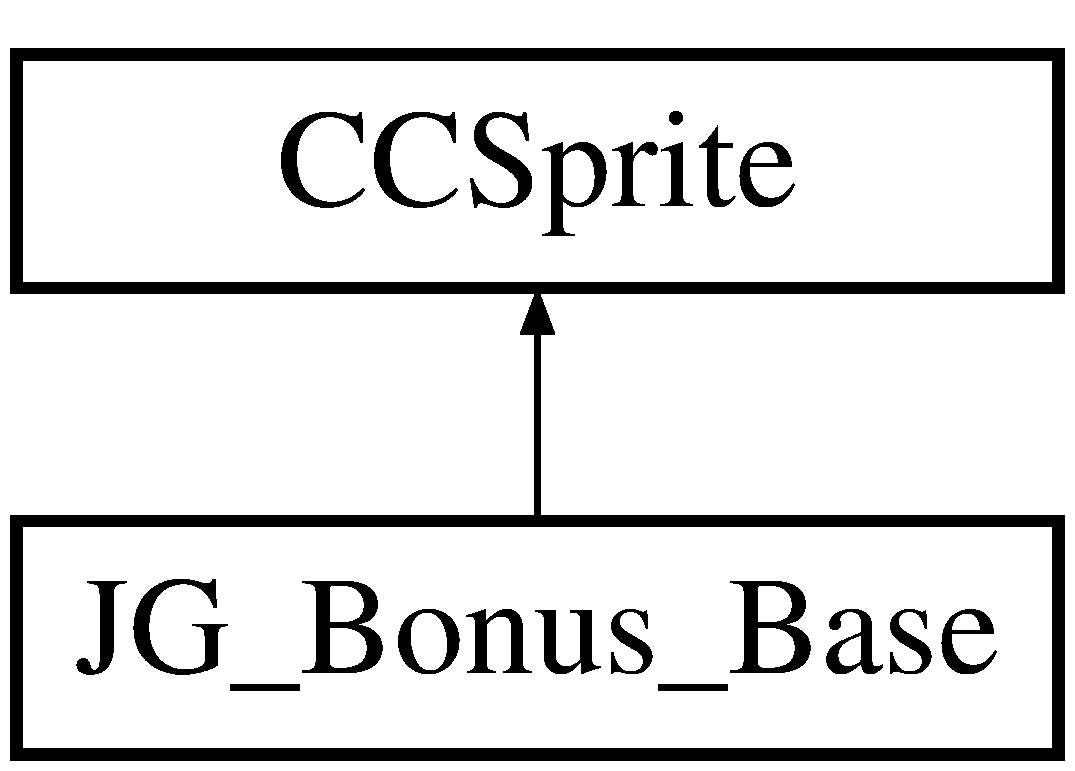
\includegraphics[height=2.000000cm]{class_j_g___bonus___base}
\end{center}
\end{figure}


The documentation for this class was generated from the following files\-:\begin{DoxyCompactItemize}
\item 
J\-G\-\_\-\-Bonus\-\_\-\-Base.\-h\item 
J\-G\-\_\-\-Bonus\-\_\-\-Base.\-cpp\end{DoxyCompactItemize}

\hypertarget{class_j_g___hand}{\section{J\-G\-\_\-\-Hand Class Reference}
\label{class_j_g___hand}\index{J\-G\-\_\-\-Hand@{J\-G\-\_\-\-Hand}}
}
Inheritance diagram for J\-G\-\_\-\-Hand\-:\begin{figure}[H]
\begin{center}
\leavevmode
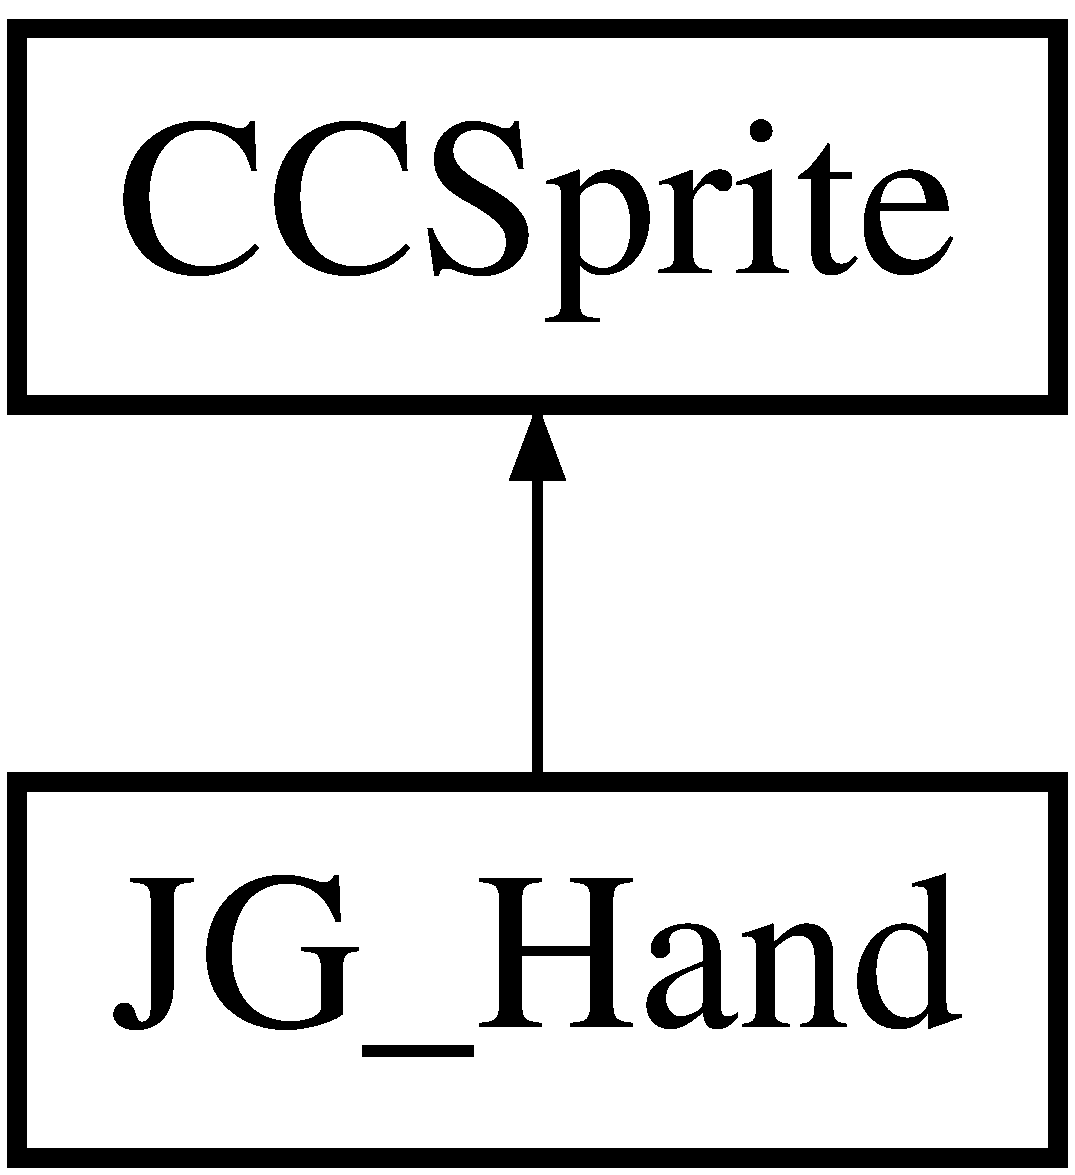
\includegraphics[height=2.000000cm]{class_j_g___hand}
\end{center}
\end{figure}
\subsection*{Public Member Functions}
\begin{DoxyCompactItemize}
\item 
\hypertarget{class_j_g___hand_aa66f82060cc53cf1790d2611476c76c0}{float {\bfseries Get\-Radius} ()}\label{class_j_g___hand_aa66f82060cc53cf1790d2611476c76c0}

\item 
\hypertarget{class_j_g___hand_aca220b8f6b4920e9324dd6b3e4f038ab}{{\bfseries C\-R\-E\-A\-T\-E\-\_\-\-F\-U\-N\-C} (\hyperlink{class_j_g___hand}{J\-G\-\_\-\-Hand})}\label{class_j_g___hand_aca220b8f6b4920e9324dd6b3e4f038ab}

\end{DoxyCompactItemize}
\subsection*{Static Public Member Functions}
\begin{DoxyCompactItemize}
\item 
\hypertarget{class_j_g___hand_af1e8c1afe129641193dc4f459ea3da62}{static \hyperlink{class_j_g___hand}{J\-G\-\_\-\-Hand} $\ast$ {\bfseries create\-With\-File\-Name} (const char $\ast$psz\-File\-Name, C\-C\-Point initial\-Pos)}\label{class_j_g___hand_af1e8c1afe129641193dc4f459ea3da62}

\end{DoxyCompactItemize}
\subsection*{Public Attributes}
\begin{DoxyCompactItemize}
\item 
\hypertarget{class_j_g___hand_abbebb5b5f2b897af0fa566477c817c96}{float {\bfseries radius}}\label{class_j_g___hand_abbebb5b5f2b897af0fa566477c817c96}

\end{DoxyCompactItemize}


The documentation for this class was generated from the following files\-:\begin{DoxyCompactItemize}
\item 
J\-G\-\_\-\-Hand.\-h\item 
J\-G\-\_\-\-Hand.\-cpp\end{DoxyCompactItemize}

\hypertarget{class_j_g___main___game}{\section{J\-G\-\_\-\-Main\-\_\-\-Game Class Reference}
\label{class_j_g___main___game}\index{J\-G\-\_\-\-Main\-\_\-\-Game@{J\-G\-\_\-\-Main\-\_\-\-Game}}
}


{\ttfamily \#include $<$J\-G\-\_\-\-Main\-\_\-\-Game.\-h$>$}

Inheritance diagram for J\-G\-\_\-\-Main\-\_\-\-Game\-:\begin{figure}[H]
\begin{center}
\leavevmode
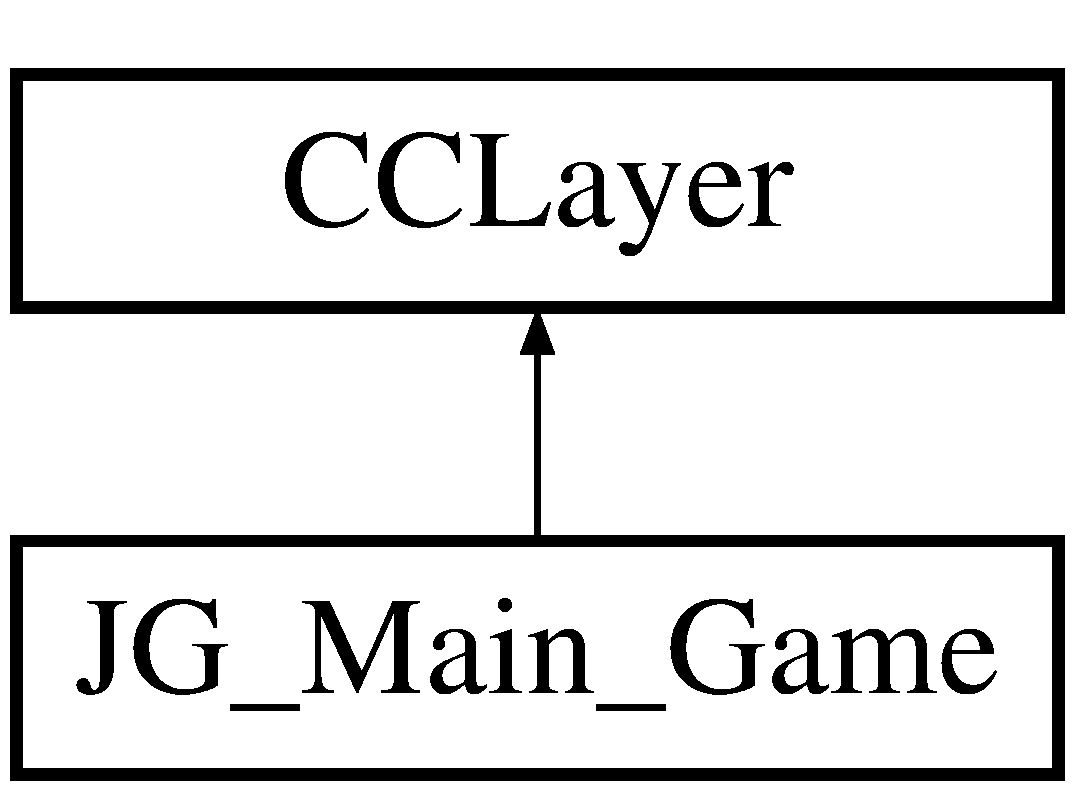
\includegraphics[height=2.000000cm]{class_j_g___main___game}
\end{center}
\end{figure}
\subsection*{Public Member Functions}
\begin{DoxyCompactItemize}
\item 
virtual bool \hyperlink{class_j_g___main___game_a9022437f7d1240ef8991b0e6c19e08ec}{init} ()
\item 
virtual void \hyperlink{class_j_g___main___game_ab4c6f1d5f85c480f1f6cd357a66cfd55}{cc\-Touches\-Began} (C\-C\-Set $\ast$p\-Touches, C\-C\-Event $\ast$event)
\item 
virtual void \hyperlink{class_j_g___main___game_a1a99f1b88de06e8882925c744be3cb91}{cc\-Touches\-Moved} (C\-C\-Set $\ast$p\-Touches, C\-C\-Event $\ast$event)
\item 
virtual void \hyperlink{class_j_g___main___game_ab9f945eff20cd58d54742828519bb6c7}{cc\-Touches\-Ended} (C\-C\-Set $\ast$p\-Touches, C\-C\-Event $\ast$event)
\item 
void \hyperlink{class_j_g___main___game_a1438760d9db28d5410b5fac68a70aa77}{update} (float dt)
\item 
bool \hyperlink{class_j_g___main___game_a92d55b1498b07adf8f83e67f71b1c7d0}{Are\-Points\-Colliding} (C\-C\-Point point1, C\-C\-Point point2, float radius)
\item 
\hypertarget{class_j_g___main___game_ae3825c2f0b5ead18bf4a7b5c8632ac9f}{void {\bfseries menu\-Close\-Callback} (C\-C\-Object $\ast$p\-Sender)}\label{class_j_g___main___game_ae3825c2f0b5ead18bf4a7b5c8632ac9f}

\item 
\hypertarget{class_j_g___main___game_af2739df486e18c008097b3e070c91ec0}{void {\bfseries menu\-Pause\-Call\-Back} (C\-C\-Object $\ast$p\-Sender)}\label{class_j_g___main___game_af2739df486e18c008097b3e070c91ec0}

\item 
\hypertarget{class_j_g___main___game_a702c39bc1dd589208b2ca832e77d5d82}{float {\bfseries get\-Sign} (float num)}\label{class_j_g___main___game_a702c39bc1dd589208b2ca832e77d5d82}

\item 
\hypertarget{class_j_g___main___game_ab9b82a7809e11b3ec224e53e06882779}{{\bfseries C\-R\-E\-A\-T\-E\-\_\-\-F\-U\-N\-C} (\hyperlink{class_j_g___main___game}{J\-G\-\_\-\-Main\-\_\-\-Game})}\label{class_j_g___main___game_ab9b82a7809e11b3ec224e53e06882779}

\item 
void \hyperlink{class_j_g___main___game_a270e423f2d88ef6c8b7151e4305f8bb5}{Test\-Touch} ()
\end{DoxyCompactItemize}
\subsection*{Static Public Member Functions}
\begin{DoxyCompactItemize}
\item 
\hypertarget{class_j_g___main___game_aacf1b844ebba39f8d75959b592557f26}{static cocos2d\-::\-C\-C\-Scene $\ast$ {\bfseries scene} ()}\label{class_j_g___main___game_aacf1b844ebba39f8d75959b592557f26}

\end{DoxyCompactItemize}


\subsection{Detailed Description}
The main class for controlling the game 

\subsection{Member Function Documentation}
\hypertarget{class_j_g___main___game_a92d55b1498b07adf8f83e67f71b1c7d0}{\index{J\-G\-\_\-\-Main\-\_\-\-Game@{J\-G\-\_\-\-Main\-\_\-\-Game}!Are\-Points\-Colliding@{Are\-Points\-Colliding}}
\index{Are\-Points\-Colliding@{Are\-Points\-Colliding}!JG_Main_Game@{J\-G\-\_\-\-Main\-\_\-\-Game}}
\subsubsection[{Are\-Points\-Colliding}]{\setlength{\rightskip}{0pt plus 5cm}bool J\-G\-\_\-\-Main\-\_\-\-Game\-::\-Are\-Points\-Colliding (
\begin{DoxyParamCaption}
\item[{C\-C\-Point}]{point1, }
\item[{C\-C\-Point}]{point2, }
\item[{float}]{radius}
\end{DoxyParamCaption}
)}}\label{class_j_g___main___game_a92d55b1498b07adf8f83e67f71b1c7d0}
checks whether distance of the two point are lesser than radius or not \hypertarget{class_j_g___main___game_ab4c6f1d5f85c480f1f6cd357a66cfd55}{\index{J\-G\-\_\-\-Main\-\_\-\-Game@{J\-G\-\_\-\-Main\-\_\-\-Game}!cc\-Touches\-Began@{cc\-Touches\-Began}}
\index{cc\-Touches\-Began@{cc\-Touches\-Began}!JG_Main_Game@{J\-G\-\_\-\-Main\-\_\-\-Game}}
\subsubsection[{cc\-Touches\-Began}]{\setlength{\rightskip}{0pt plus 5cm}void J\-G\-\_\-\-Main\-\_\-\-Game\-::cc\-Touches\-Began (
\begin{DoxyParamCaption}
\item[{C\-C\-Set $\ast$}]{p\-Touches, }
\item[{C\-C\-Event $\ast$}]{event}
\end{DoxyParamCaption}
)\hspace{0.3cm}{\ttfamily [virtual]}}}\label{class_j_g___main___game_ab4c6f1d5f85c480f1f6cd357a66cfd55}
Handles the beginning of the touch \hypertarget{class_j_g___main___game_ab9f945eff20cd58d54742828519bb6c7}{\index{J\-G\-\_\-\-Main\-\_\-\-Game@{J\-G\-\_\-\-Main\-\_\-\-Game}!cc\-Touches\-Ended@{cc\-Touches\-Ended}}
\index{cc\-Touches\-Ended@{cc\-Touches\-Ended}!JG_Main_Game@{J\-G\-\_\-\-Main\-\_\-\-Game}}
\subsubsection[{cc\-Touches\-Ended}]{\setlength{\rightskip}{0pt plus 5cm}void J\-G\-\_\-\-Main\-\_\-\-Game\-::cc\-Touches\-Ended (
\begin{DoxyParamCaption}
\item[{C\-C\-Set $\ast$}]{p\-Touches, }
\item[{C\-C\-Event $\ast$}]{event}
\end{DoxyParamCaption}
)\hspace{0.3cm}{\ttfamily [virtual]}}}\label{class_j_g___main___game_ab9f945eff20cd58d54742828519bb6c7}
Handles the end of the touch \hypertarget{class_j_g___main___game_a1a99f1b88de06e8882925c744be3cb91}{\index{J\-G\-\_\-\-Main\-\_\-\-Game@{J\-G\-\_\-\-Main\-\_\-\-Game}!cc\-Touches\-Moved@{cc\-Touches\-Moved}}
\index{cc\-Touches\-Moved@{cc\-Touches\-Moved}!JG_Main_Game@{J\-G\-\_\-\-Main\-\_\-\-Game}}
\subsubsection[{cc\-Touches\-Moved}]{\setlength{\rightskip}{0pt plus 5cm}void J\-G\-\_\-\-Main\-\_\-\-Game\-::cc\-Touches\-Moved (
\begin{DoxyParamCaption}
\item[{C\-C\-Set $\ast$}]{p\-Touches, }
\item[{C\-C\-Event $\ast$}]{event}
\end{DoxyParamCaption}
)\hspace{0.3cm}{\ttfamily [virtual]}}}\label{class_j_g___main___game_a1a99f1b88de06e8882925c744be3cb91}
Handles the movement of the touch \hypertarget{class_j_g___main___game_a9022437f7d1240ef8991b0e6c19e08ec}{\index{J\-G\-\_\-\-Main\-\_\-\-Game@{J\-G\-\_\-\-Main\-\_\-\-Game}!init@{init}}
\index{init@{init}!JG_Main_Game@{J\-G\-\_\-\-Main\-\_\-\-Game}}
\subsubsection[{init}]{\setlength{\rightskip}{0pt plus 5cm}bool J\-G\-\_\-\-Main\-\_\-\-Game\-::init (
\begin{DoxyParamCaption}
{}
\end{DoxyParamCaption}
)\hspace{0.3cm}{\ttfamily [virtual]}}}\label{class_j_g___main___game_a9022437f7d1240ef8991b0e6c19e08ec}
Initial the game state \hypertarget{class_j_g___main___game_a270e423f2d88ef6c8b7151e4305f8bb5}{\index{J\-G\-\_\-\-Main\-\_\-\-Game@{J\-G\-\_\-\-Main\-\_\-\-Game}!Test\-Touch@{Test\-Touch}}
\index{Test\-Touch@{Test\-Touch}!JG_Main_Game@{J\-G\-\_\-\-Main\-\_\-\-Game}}
\subsubsection[{Test\-Touch}]{\setlength{\rightskip}{0pt plus 5cm}void J\-G\-\_\-\-Main\-\_\-\-Game\-::\-Test\-Touch (
\begin{DoxyParamCaption}
{}
\end{DoxyParamCaption}
)}}\label{class_j_g___main___game_a270e423f2d88ef6c8b7151e4305f8bb5}
a function to test touch \hypertarget{class_j_g___main___game_a1438760d9db28d5410b5fac68a70aa77}{\index{J\-G\-\_\-\-Main\-\_\-\-Game@{J\-G\-\_\-\-Main\-\_\-\-Game}!update@{update}}
\index{update@{update}!JG_Main_Game@{J\-G\-\_\-\-Main\-\_\-\-Game}}
\subsubsection[{update}]{\setlength{\rightskip}{0pt plus 5cm}void J\-G\-\_\-\-Main\-\_\-\-Game\-::update (
\begin{DoxyParamCaption}
\item[{float}]{dt}
\end{DoxyParamCaption}
)}}\label{class_j_g___main___game_a1438760d9db28d5410b5fac68a70aa77}
update function 

The documentation for this class was generated from the following files\-:\begin{DoxyCompactItemize}
\item 
J\-G\-\_\-\-Main\-\_\-\-Game.\-h\item 
J\-G\-\_\-\-Main\-\_\-\-Game.\-cpp\end{DoxyCompactItemize}

\hypertarget{class_j_g___main___menu}{\section{J\-G\-\_\-\-Main\-\_\-\-Menu Class Reference}
\label{class_j_g___main___menu}\index{J\-G\-\_\-\-Main\-\_\-\-Menu@{J\-G\-\_\-\-Main\-\_\-\-Menu}}
}
Inheritance diagram for J\-G\-\_\-\-Main\-\_\-\-Menu\-:\begin{figure}[H]
\begin{center}
\leavevmode
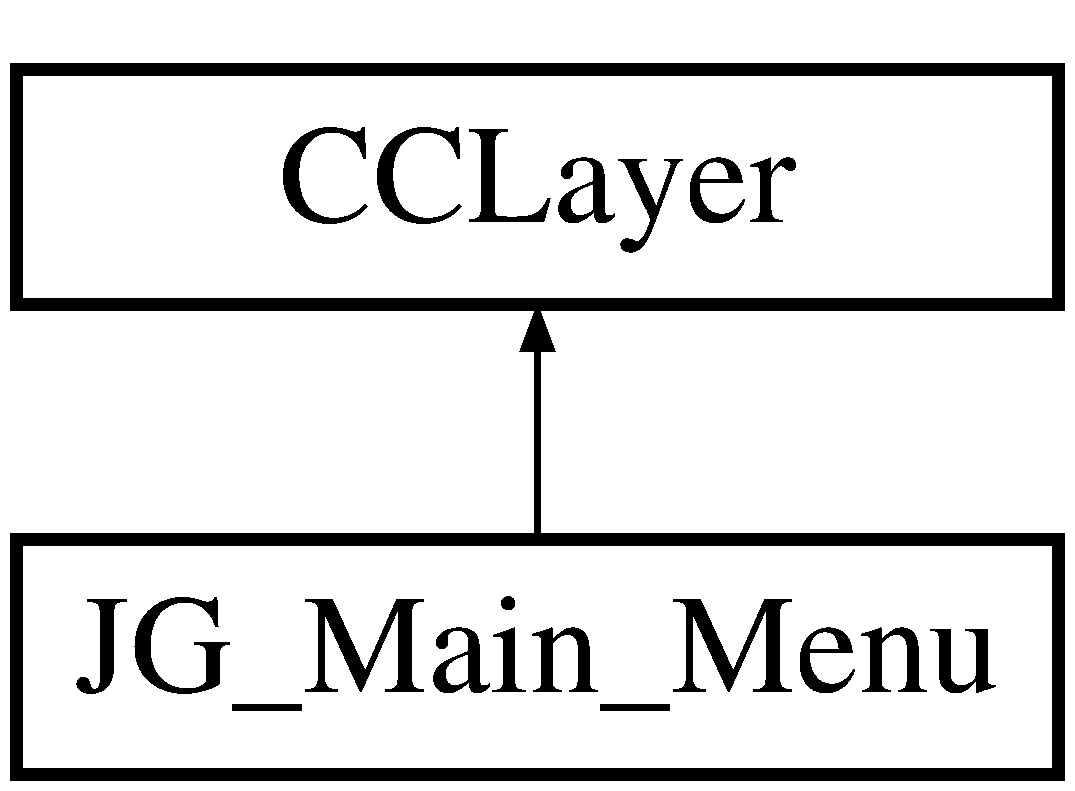
\includegraphics[height=2.000000cm]{class_j_g___main___menu}
\end{center}
\end{figure}
\subsection*{Public Member Functions}
\begin{DoxyCompactItemize}
\item 
\hypertarget{class_j_g___main___menu_a93b78909b38318f329a517fd62de1277}{virtual bool {\bfseries init} ()}\label{class_j_g___main___menu_a93b78909b38318f329a517fd62de1277}

\item 
\hypertarget{class_j_g___main___menu_a5bb79dee5a63aeb889c7033b7f0c8074}{void {\bfseries menu\-Close\-Callback} (C\-C\-Object $\ast$p\-Sender)}\label{class_j_g___main___menu_a5bb79dee5a63aeb889c7033b7f0c8074}

\item 
\hypertarget{class_j_g___main___menu_a26e1d7c8a1924315b6e6099da52a30af}{void {\bfseries menu\-Pause\-Call\-Back} (C\-C\-Object $\ast$p\-Sender)}\label{class_j_g___main___menu_a26e1d7c8a1924315b6e6099da52a30af}

\item 
\hypertarget{class_j_g___main___menu_abd196eed8a51b71deb76bd778ad03adf}{{\bfseries C\-R\-E\-A\-T\-E\-\_\-\-F\-U\-N\-C} (\hyperlink{class_j_g___main___menu}{J\-G\-\_\-\-Main\-\_\-\-Menu})}\label{class_j_g___main___menu_abd196eed8a51b71deb76bd778ad03adf}

\end{DoxyCompactItemize}
\subsection*{Static Public Member Functions}
\begin{DoxyCompactItemize}
\item 
\hypertarget{class_j_g___main___menu_a600962585d8d197284ea6ff04a8caca8}{static cocos2d\-::\-C\-C\-Scene $\ast$ {\bfseries scene} ()}\label{class_j_g___main___menu_a600962585d8d197284ea6ff04a8caca8}

\end{DoxyCompactItemize}


The documentation for this class was generated from the following files\-:\begin{DoxyCompactItemize}
\item 
J\-G\-\_\-\-Main\-\_\-\-Menu.\-h\item 
J\-G\-\_\-\-Main\-\_\-\-Menu.\-cpp\end{DoxyCompactItemize}

\hypertarget{class_j_g___temp_line_container}{\section{J\-G\-\_\-\-Temp\-Line\-Container Class Reference}
\label{class_j_g___temp_line_container}\index{J\-G\-\_\-\-Temp\-Line\-Container@{J\-G\-\_\-\-Temp\-Line\-Container}}
}
Inheritance diagram for J\-G\-\_\-\-Temp\-Line\-Container\-:\begin{figure}[H]
\begin{center}
\leavevmode
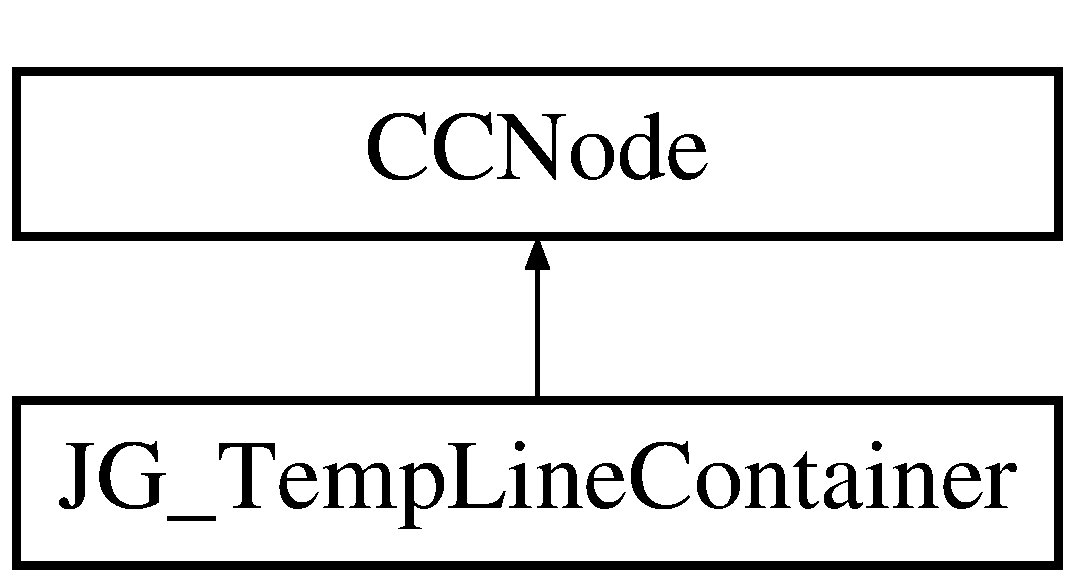
\includegraphics[height=2.000000cm]{class_j_g___temp_line_container}
\end{center}
\end{figure}
\subsection*{Public Member Functions}
\begin{DoxyCompactItemize}
\item 
\hypertarget{class_j_g___temp_line_container_a76d934621da27e6655c82fa3f47367fb}{{\bfseries C\-C\-\_\-\-S\-Y\-N\-T\-H\-E\-S\-I\-Z\-E} (float, \-\_\-energy, Energy)}\label{class_j_g___temp_line_container_a76d934621da27e6655c82fa3f47367fb}

\item 
\hypertarget{class_j_g___temp_line_container_a000b563cdf4514db05690c6a5a58bf8f}{{\bfseries C\-C\-\_\-\-S\-Y\-N\-T\-H\-E\-S\-I\-Z\-E} (C\-C\-Point, \-\_\-pivot, Pivot)}\label{class_j_g___temp_line_container_a000b563cdf4514db05690c6a5a58bf8f}

\item 
\hypertarget{class_j_g___temp_line_container_ac08d97e1c2aec33333af36d4a6bb082a}{{\bfseries C\-C\-\_\-\-S\-Y\-N\-T\-H\-E\-S\-I\-Z\-E} (C\-C\-Point, \-\_\-tip, Tip)}\label{class_j_g___temp_line_container_ac08d97e1c2aec33333af36d4a6bb082a}

\item 
\hypertarget{class_j_g___temp_line_container_aec49e4d98621fc93f88c86a0d8c9106f}{{\bfseries C\-C\-\_\-\-S\-Y\-N\-T\-H\-E\-S\-I\-Z\-E} (float, \-\_\-line\-Length, Line\-Length)}\label{class_j_g___temp_line_container_aec49e4d98621fc93f88c86a0d8c9106f}

\item 
\hypertarget{class_j_g___temp_line_container_abeee2ee1f80e70f392d9565221da2312}{{\bfseries C\-C\-\_\-\-S\-Y\-N\-T\-H\-E\-S\-I\-Z\-E} (Line\-Type, \-\_\-line\-Type, Line\-Type)}\label{class_j_g___temp_line_container_abeee2ee1f80e70f392d9565221da2312}

\item 
\hypertarget{class_j_g___temp_line_container_a36203326958031be1c0ff7a3cc61d2eb}{virtual void {\bfseries draw} ()}\label{class_j_g___temp_line_container_a36203326958031be1c0ff7a3cc61d2eb}

\item 
\hypertarget{class_j_g___temp_line_container_a3fd0208929faccbff7e44ed5bfdad197}{void {\bfseries update} (float dt)}\label{class_j_g___temp_line_container_a3fd0208929faccbff7e44ed5bfdad197}

\item 
\hypertarget{class_j_g___temp_line_container_a92c74cc9ad1a56fb2b974b2eaa93d2f9}{void {\bfseries set\-Energy\-Decrement} (float value)}\label{class_j_g___temp_line_container_a92c74cc9ad1a56fb2b974b2eaa93d2f9}

\item 
\hypertarget{class_j_g___temp_line_container_aad9a9bee32831fff0cb4b03877616913}{void {\bfseries reset} (void)}\label{class_j_g___temp_line_container_aad9a9bee32831fff0cb4b03877616913}

\end{DoxyCompactItemize}
\subsection*{Static Public Member Functions}
\begin{DoxyCompactItemize}
\item 
\hypertarget{class_j_g___temp_line_container_a0b2d8c7545456651abc6d5f60a690a14}{static \hyperlink{class_j_g___temp_line_container}{J\-G\-\_\-\-Temp\-Line\-Container} $\ast$ {\bfseries create} ()}\label{class_j_g___temp_line_container_a0b2d8c7545456651abc6d5f60a690a14}

\end{DoxyCompactItemize}


The documentation for this class was generated from the following files\-:\begin{DoxyCompactItemize}
\item 
J\-G\-\_\-\-Temp\-Line\-Container.\-h\item 
J\-G\-\_\-\-Temp\-Line\-Container.\-cpp\end{DoxyCompactItemize}

%--- End generated contents ---

% Index
\newpage
\phantomsection
\addcontentsline{toc}{part}{Index}
\printindex

\end{document}
